\documentclass[tikz,border=10pt]{standalone}
\usepackage{tikz}
\begin{document}
% Örnek 1
\begin{tikzpicture}
\draw (0,0) -- (1,1);
\end{tikzpicture}

% Örnek 2
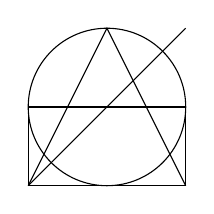
\begin{tikzpicture}
\draw (0,0) -- (2,2); % İki nokta arasında düz bir çizgi çizer
\draw (0,0) rectangle (2,1); % Dikdörtgen çizer
\draw (1,1) circle (1cm); % Yarıçapı 1 cm olan bir daire çizer
\draw (0,0) -- (1,2) -- (2,0); % Çokgen çizer
\end{tikzpicture}

\end{document}
